\documentclass{llncs}

\usepackage[utf8]{inputenc}
\usepackage[T1]{fontenc}

% \usepackage{amsmath}
% \usepackage{amssymb}
% \usepackage{amsthm}
% \usepackage{xspace}
% \usepackage{todonotes}
% \usepackage{authblk}
\usepackage{graphicx}
\usepackage{listings}
% \usepackage{wrapfig}
% \usepackage[inline,shortlabels]{enumitem}

\usepackage{cite} % sort cite numbers, prevent breaks
\usepackage{fnpct} % nicely typeset footnotes *preceding* punctuation
\usepackage{microtype} % towards typographic perfection

\usepackage{hyperref}
\usepackage{cleveref}

\widowpenalty1000
\clubpenalty1000

\title{odgf-python -- A Python Interface for the Open Graph Drawing~Framework%
  \thanks{Funded by the Deutsche Forschungsgemeinschaft (German Research Foundation, DFG) under grant RU-1903/3-1.}
}
\author{Simon D. Fink\orcidID{0000-0002-2754-1195}, Andreas Strobl}
\institute{Faculty for Mathematics and Computer Science, University of Passau,\\Passau, Germany\\\email{\{finksim,strobland\}@fim.uni-passau.de}}
\date{}

\begin{document}

\maketitle

\begin{abstract}
The Open Graph Drawing Framework (OGDF) is a C++ library that contains a vast amount of algorithms and data structures for automatic graph drawing.
While the library is powerful, it is also not easily accessible for new users and the nature of C++ makes implementing even simple algorithms cumbersome to non-experts.
The \texttt{odgf-python} project remedies these problems by making the full functionality of the OGDF available from Python, providing a visual way to iteratively develop graph algorithms.

\keywords {OGDF \and Graph Algorithms \and Python \and Jupyter Notebooks}
\end{abstract}


The Open Graph Drawing Framework (OGDF) \cite{cgj-tog-13} is a C++ library that contains a vast amount of algorithms and data structures for
automatic graph drawing.
While the library is powerful, it is also not easily accessible for new users and the nature of C++ makes implementing even simple algorithms cumbersome to non-experts.
New C++ projects require non-trivial set-up and distinct code-compile-execute iterations make it hard to incrementally develop a new algorithm.
This is because they separate the code from its results and there is no easy way to debug and visually analyze the current state of the program.

Many of these issues have been resolved within the Python ecosystem \cite{per-tcc-21}.
The \texttt{odgf-python}\footnote{\url{https://github.com/N-Coder/ogdf-python}} project remedies these problems also for the OGDF by making its full functionality available from Python.
A similar approach has recently been taken to make the Computational Geometry Algorithms Library (CGAL) more accessible \cite{gfh-cmm-22}.
A Python interface greatly reduces the overhead and complications when using a library for the first time and unlocks a large ecosystem
of other libraries and tools, for example the interactive computing Notebooks provided by Project Jupyter \cite{krp-jn-16}.
These Notebooks allow iteratively developing algorithms and visualize their results inline right next to their code \cite{per-tcc-21}.
They are widely used in different scientific contexts and constitute the de facto standard in data science \cite{per-wji-18}.

A key component of the \texttt{odgf-python} library is its graph display widget for Jupyter Notebooks \cite{str-agw-22}.
It can be used as-is to quickly explore and modify the current graph in-memory.
At the same time, it can be used as a building block for more complex user interfaces, where its interactivity can be fully customized to suit different applications.
Combining this with the UI components of Jupyter's \texttt{ipywidgets} allows to easily build platform-independent user interfaces for interacting with graphs and algorithms.
Example use cases include the iterative development of new graph algorithms,
step-by-step debugging of implemented algorithms,
visual editing of in-memory graphs and variables,
interactive visualization of algorithms for teaching, and 
flexible user interfaces for domain-specific applications.

Internally, \texttt{ogdf-python} uses the \texttt{cppyy} library \cite{ld-hpp-16,kvl-eaa-23} to automatically generate python bindings for the C++ OGDF library.
One of the main advantages of \texttt{cppyy} is that there is no need for explicitly declared bindings or interfaces.
This makes \texttt{ogdf-python} future-proof by being automatically compatible with future versions of the OGDF without the need for adaptions or manual updates to declarations.
The \texttt{cppyy} library also allows for arbitrary C++ code to be loaded and called from Python.
This allows for variables, functions and even classes to be created and used in either language.

\subsection*{Features}
\begin{itemize}
\item \textbf{No C++ skills needed}: The full OGDF API is available from Python.
\item \textbf{Rapid prototyping}: Python needs less boilerplate and allows more idiomatic constructions, 
  without the need to configure and compile anything.
\item \textbf{Iterative execution}: Jupyter Notebooks allow individual lines of code to be adapted and re-run,
  retaining all previous variable values.
\item \textbf{Inline results}: Graphs are visually displayed right next to the code that generates them.
\item \textbf{Interactive graph exploration}: The inline display allows interactive zooming and panning to easily explore the graph.
\item \textbf{Extensible building block}: The library can be easily combined with other projects from the Python ecosystem, for example with \texttt{ipywidgets} to build portable user interfaces for graphs.
\end{itemize}

\subsection*{Installation}
The \texttt{ogdf-python} library comes with a prebuilt version of the OGDF called \texttt{ogdf-wheel} that works on Linux, macOS and in the Windows Subsystem for Linux.
Both components can easily be installed using the Python package manager~pip:

\begin{lstlisting}[language=bash]
pip3 install ogdf-python ogdf-wheel notebook
jupyter notebook # start an interactive notebook
\end{lstlisting}

% \begin{figure}[h]
%   \centering
%   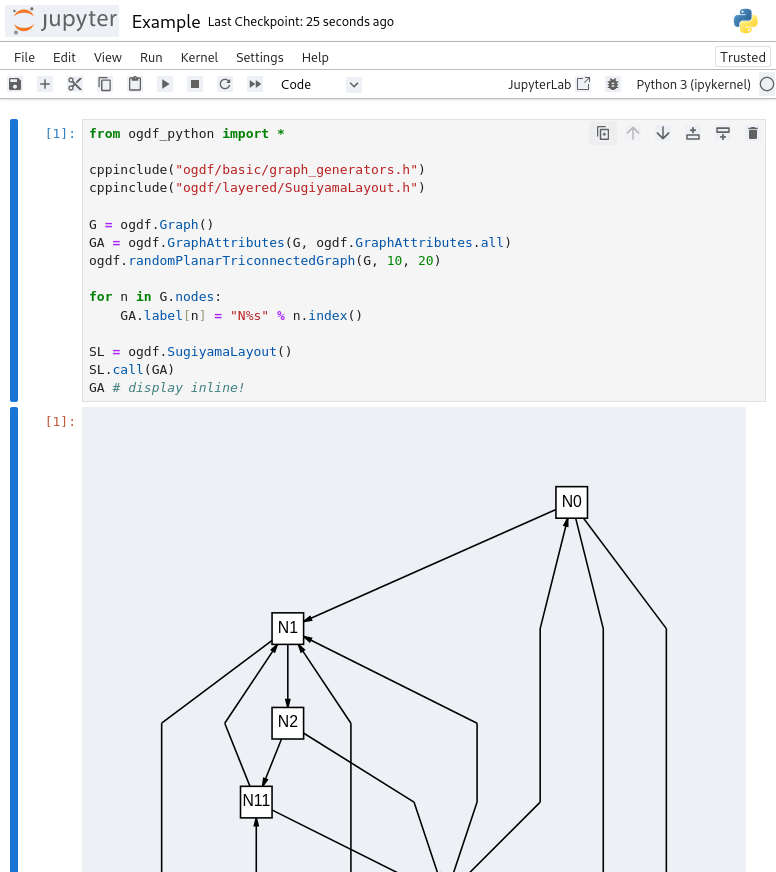
\includegraphics[width=.5\linewidth]{screenshot}
%   \caption{A screenshot of a Jupyter Notebook with some example code using \texttt{ogdf-python} followed by an inline visualization of its resulting graph layout.}
%   \label{fig}
% \end{figure}

\bibliographystyle{splncs04}
\bibliography{bibliography}

\end{document}
